\documentclass[a4paper,10pt,oneside,final]{article}


\usepackage[english]{babel}
\usepackage[T1]{fontenc}
\usepackage{tabularx}
\usepackage[usenames,dvipsnames]{color}
\usepackage[table]{xcolor}
\usepackage[left=3.0cm, right=2.5cm, top=2.5cm, bottom=2.5cm]{geometry}
\usepackage{graphicx}
\usepackage{float}
\usepackage{caption}
\usepackage{listings}


\lstdefinestyle{ccc} 
{ 
numbers=none, 
basicstyle=\small\ttfamily, 
keywordstyle=\bf\color[rgb]{0,0,0}, 
%commentstyle=\color[rgb]{0.133,0.545,0.133}, 
stringstyle=\color[rgb]{0.627,0.126,0.941}, 
backgroundcolor=\color{white}, 
frame=tb, %frame= lrtb, 
framerule=0.5pt, 
linewidth=\textwidth,
%aboveskip=-4.0pt,
%belowskip=-4.0pt,
lineskip=-5.0pt,
}

%
% Define author(s) and  component's name
%
\def\defauthor{Lasse Lehtonen}
\def\deftitle{FH Mesh\_2D\\Reference Manual}



\author{\defauthor}
\title{\deftitle}

\usepackage{fancyhdr} 
\pagestyle{fancy} 
\lhead{\bfseries Department of Computer Systems\\
  Faculty of Computing and Electrical Engineering}
\chead{} 
\rhead{\bfseries \deftitle} 
\lfoot{\thepage} 
\cfoot{}
\rfoot{
\includegraphics[height=1.0cm]{pic/tty_logo.png}}
\renewcommand{\headrulewidth}{0.4pt}
\renewcommand{\footrulewidth}{0.4pt}


\def\deftablecolora{blue!10!white}
\def\deftablecolorb{white}

\begin{document}


%\maketitle
%\thispagestyle{empty}

\begin{titlepage}
\begin{center}

\vspace{6.0cm}
\textsc{\LARGE Tampere University of Technology}\\[1.0cm]
\textsc{\Large Faculty of Computing and Electrical Engineering}\\[1.0cm]
\textsc{\Large Department of Computer Systems}\\[1.0cm]
\vspace{6.0cm}
\hrule
\vspace{0.4cm}
{ \huge \bfseries FH Mesh\_2D\\[0.5cm]Reference Manual}
\vspace{0.4cm}
\hrule

%\vspace{2.0cm}

\vfill

\begin{minipage}{0.4\textwidth}
\begin{flushleft} \large
\emph{Author:}\\
Lasse Lehtonen
\end{flushleft}
\end{minipage}
\begin{minipage}{0.4\textwidth}
\begin{flushright} \large
\emph{Updated:} \\
\today
\end{flushright}
\end{minipage}

\end{center}
\end{titlepage}

\newpage
\tableofcontents



\newpage
\section{REVISION HISTORY}
\setcounter{page}{1}

\begin{center}
  \rowcolors{3}{\deftablecolora}{\deftablecolorb}
  
  \captionof{table}{}
  \begin{tabularx}{\textwidth}{|lllX|}
    \hline
    Revision & Author          & Date       & Description\\
    \hline
    1.00  & Lasse Lehtonen  & 8.8.2011 & Initial documentation\\
    & & & \\
    & & & \\
    & & & \\
    & & & \\
    \hline
  \end{tabularx}
\end{center}



\newpage
\section{DOCUMENT OVERVIEW}

\subsection{SCOPE}

This documentation describes the basic operation and usage of FH
Mesh\_2D Network-on-Chip component.

\subsection{AUDIENCE}

For hardware integrators wanting to use this component.

\subsection{RELATED DOCUMENTATION}

\begin{center}
  \rowcolors[]{2}{\deftablecolora}{\deftablecolorb}

  \captionof{table}{}
  \begin{tabularx}{\textwidth}{|lX|}
    \hline
    Document & Description\\
    \hline    
    & \\
    & \\
    & \\
    & \\
    \hline
  \end{tabularx}
\end{center}

\subsection{DOCUMENT CONVENTIONS}


\begin{itemize}
\item Ports: \texttt{teletype} in text
\item Generics: \texttt{teletype} in text
\end{itemize}



\newpage
\section{INTRODUCTION}

\subsection{BRIEF DESCRIPTION}

FH Mesh\_2D Network-on-Chip is a highly configurable network based on
2-dimensional mesh architecture. Network can be configured to use
either store-and-forward of wormhole switching, but is limited to only
XY routing. Fifo depths and bus widths can be freely set and the
network supports different synchronous frequencies for agents than the
network's operating frequency.

\subsection{EXAMPLE SYSTEM}

Example system in figure~\ref{fig:example_system} presents a 5 by 4
mesh topology. Every router is connected to one agent and all
neighboring routers in cardinal directions with bi-directional links.

\begin{center}  
  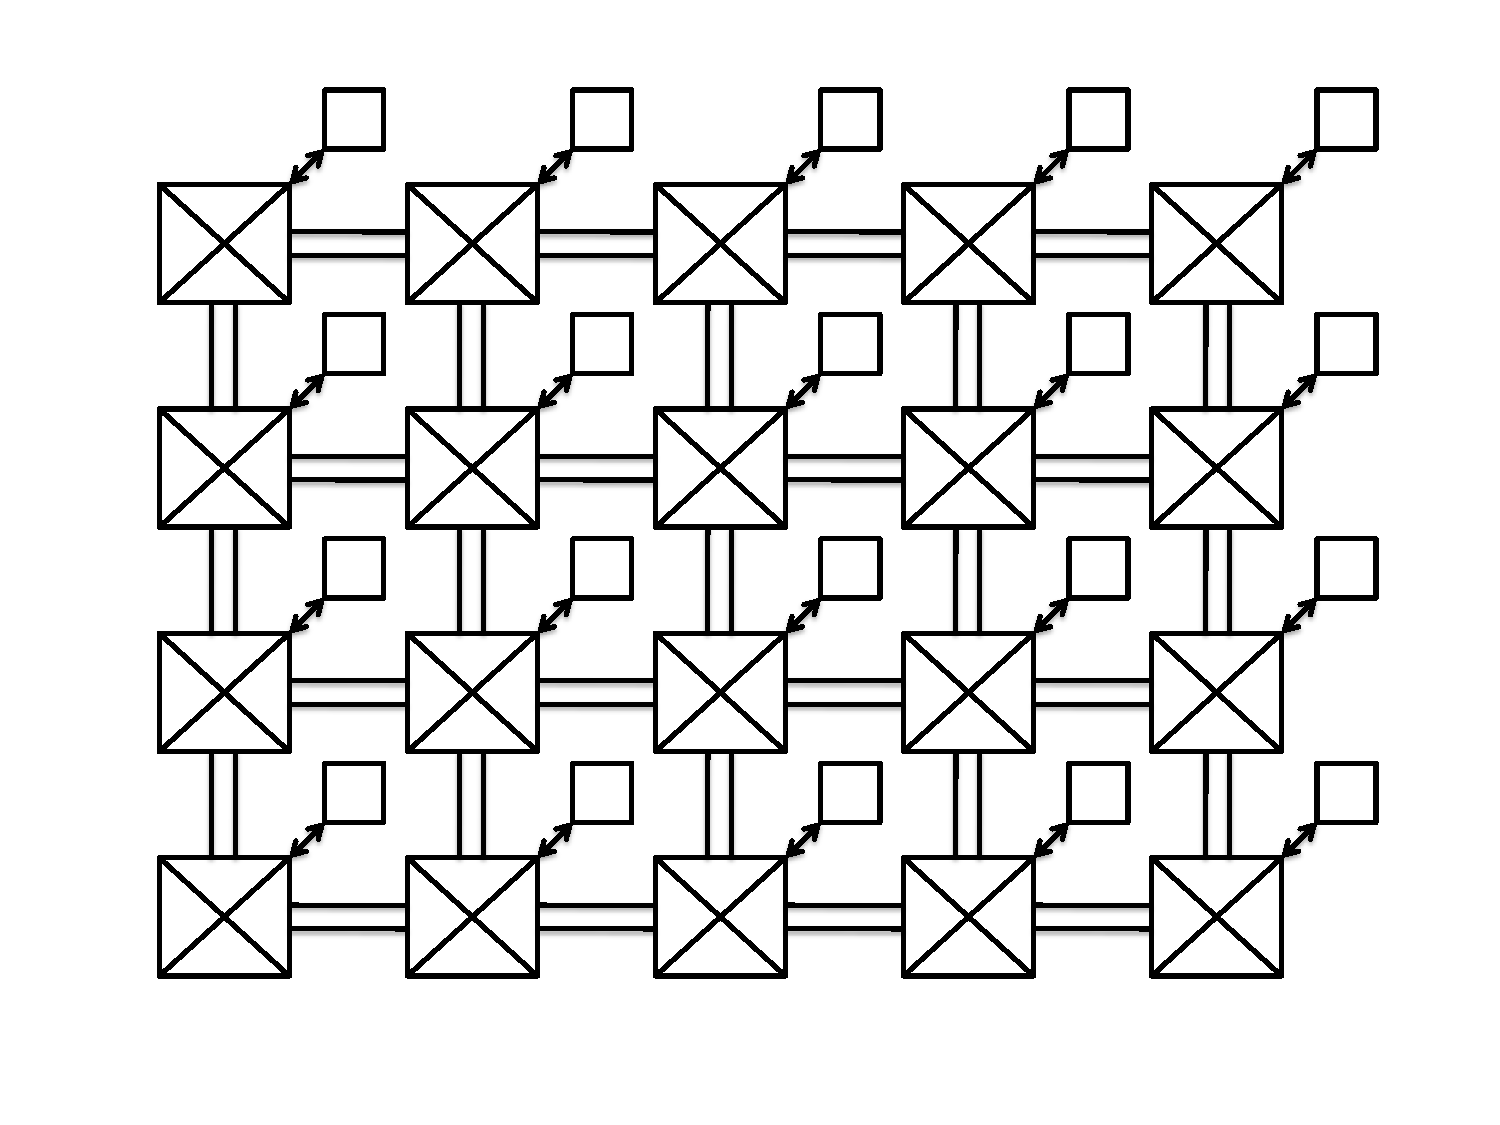
\includegraphics[width=1.0\textwidth]{pic/mesh_5x4.pdf}
  \captionof{figure}{}  
  \label{fig:example_system}
\end{center}



\newpage
\section{HARDWARE DESIGN}

\subsection{FH MESH\_2D}

\subsubsection{GENERICS}

\begin{center}
  \rowcolors{3}{\deftablecolora}{\deftablecolorb}

  \captionof{table}{}
  \begin{tabularx}{\textwidth}{|lX|}
    \hline
    Name                & Description\\
    \hline
    n\_ag\_g          & Number of agents\\
    stfwd\_en\_g      & Selects between store-and-forward (1) 
                          and wormhole (0) switching\\
    data\_width\_g    & Width of the data bus in bits\\
    addr\_width\_g    & Width of the address bus in bits. Must be less 
                          or equal than data\_width\_g\\
    tx\_len\_width\_g & Width of txlen bus in bits\\
    packet\_length\_g & Packet's maximum length in words\\
    timeout\_g        & How many clock cycles to wait for packet to fill
                        before filling it with dummy data\\
    lut\_en\_g        & Enable address translation\\
    fifo\_depth\_g    & Depth of FIFOs in words\\
    len\_flit\_en\_g  & Enable packet to carry length information in 
                           its own flit\\
    oaddr\_flit\_en\_g & Enable packet to carry the destination 
                             memory-mapped address\\
    mesh\_freq\_g  & Network's frequency relative to IP  frequecy\\
    ip\_freq\_g    & Agent's relative frequency to network frequecy\\
    rows\_g & Number of rows in the network\\
    cols\_g & Number of columns in the network\\
    \hline
  \end{tabularx}
\end{center}

\subsubsection{CLOCKING AND RESET}


\begin{center}
  \rowcolors{3}{\deftablecolora}{\deftablecolorb}

  \captionof{table}{}
  \begin{tabularx}{\textwidth}{|lllX|}
    \hline
    Port   & Width & Direction & Description\\
    \hline
    clk\_mesh    & 1     & in      & Clock for the network, active on rising edge\\
    clk\_ip    & 1     & in      & Clock for the IP, active on rising edge\\
    rst\_n & 1     & in      & Reset, asynchronous, active low\\
    \hline
  \end{tabularx}
\end{center}

Clock frequencies must be at integer ratio (e.g. 1:3 but not 2:3) and they must
have a synchronized rising edge.

\subsubsection{DATA INTERFACE}

\begin{center}
  \rowcolors{3}{\deftablecolora}{\deftablecolorb}

  \captionof{table}{}
  \begin{tabularx}{\textwidth}{|lllX|}
    \hline
    Port   & Width & Direction & Description\\
    \hline
    tx\_data\_in & rows\_g*cols\_g*data\_width\_g & in  & All TX datas from IPs \\
    tx\_we\_in & rows\_g*cols\_g & in & Write enables from all IPs\\
    tx\_txlen\_in & rows\_g*cols\_g*tx\_len\_width\_g & in & Transfer's length in words\\
    rx\_re\_in & rows\_g*cols\_g & in & Read enables from all IPs\\
    rx\_data\_out & rows\_g*cols\_g*data\_width\_g & out & All RX datas from the network\\
    rx\_empty\_out & rows\_g*cols\_g & out &  RX FIFO empty signals\\
    rx\_full\_out & rows\_g*cols\_g & out &  RX FIFO full signals\\
    tx\_empty\_out & rows\_g*cols\_g & out &  TX FIFO empty signals\\
    tx\_full\_out & rows\_g*cols\_g & out &  TX FIFO full signals\\
    \hline
  \end{tabularx}
\end{center}

Routers are connected to vectors starting from $(X=0, Y=0)$ and continuing
row by row from $X=0$ to $X=cols\_g-1$.



\subsubsection{ARCHITECTURE}

Router design contains a basic synchronous FIFO for incoming links on
cardinal directions and multiclock FIFOs capable of synchronous clock
domain crossing for both ways connected to the Packet Codec. Packet
codec acts as network interface for IPs handling the creation of
packets and the address translation from memory mapped addresses to
network addresses.

\begin{center}  
  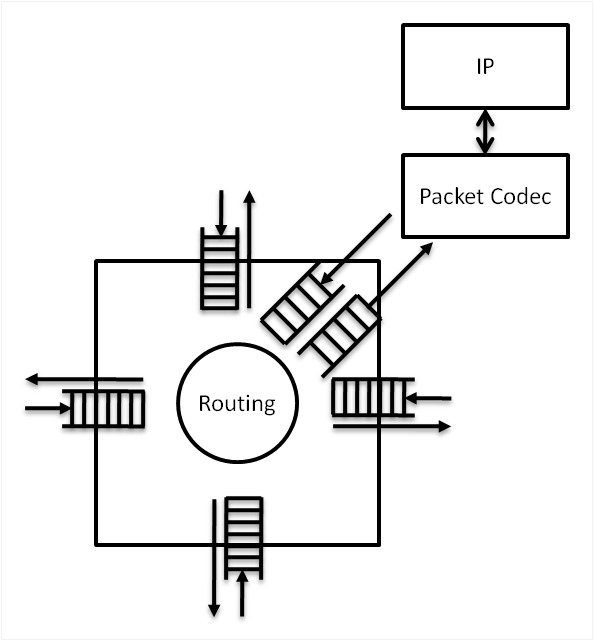
\includegraphics[width=0.4\textwidth]{pic/router_arch.png}
  \captionof{figure}{}
\end{center}

\subsubsection{INTEGRATION}

Related  source  files  are listed  in  next  table  in the  order  of
compilation (when applicable).

\begin{center}
  \rowcolors{3}{\deftablecolora}{\deftablecolorb}

  \captionof{table}{}
  \label{tab:files}
  \begin{tabularx}{\textwidth}{|lX|}
    \hline
    Filename   & Description\\
    \hline
    fifo.vhd           & Simple synchronous FIFO\\
    multiclk\_fifo.vhd & FIFO with clock domain crossing\\
    pkt\_counter.vhd   & Debug component counting packets\\   
    addr\_lut\_pkg.vhd & Package for pkt\_codec\\
    addr\_lut.vhd      & Address translation unit\\
    pkt\_enc.vhd       & Packet encoder\\
    pkt\_dec.vhd       & Pakcet decoder\\
    pkt\_enc\_dec\_1d  & Top level for encoders and decoders\\    
    mesh\_router.vhd   & Router implementation\\
    mesh\_2d.vhd       & Top level containing all routers\\
    mesh\_2d\_with\_pkt\_codec\_top.vhd & Top level with pkt\_codec\\
    \hline
  \end{tabularx}  
\end{center}


\subsubsection{SWITCHING}

Depending on generic \texttt{stfwd\_en\_g} FH Mesh\_2D uses either
store-and-forward or wormhole switching. If store-and-forward
switching is used the Packet Codec handles the creation of the
network packet. If there's not enough data to fill the whole packet
the unused flits will be sent empty. Packet Codec will wait few clock
cycles before filling the packet to allow IP to stall a little while
sending. For store-and-forward switching the FIFOs must be the same
size as the packets. 

\vspace{0.4cm}
\noindent
For wormhole switched configuration there's no limitation to the size
of the FIFOs.


\subsubsection{ROUTING}

Routing algorithm of FH Mesh\_2D if fixed to YX-routing. Packets travel
first on the Y-axis to the correct row and then along the X-axis to
the destination router.

\newpage
\section{TESTING}

\subsection{TEST CASE}

FH Mesh\_2D network model comes with a simple test case which instantiates
a 2 by 3 mesh with packet codec inteface. Test case sends one message
from router (0,0) to router (1,2) and terminates after that.

\subsection{SIMULATION}

In order to simulate the test case one needs to compile files listed
in table~\ref{tab:files} in addition to files listed in
table~\ref{tab:simfiles} found in basic\_tester/vhd. Top level for the
simulation (simple\_test\_mesh\_2d.vhd) and the test case files are
located in directory mesh\_2d/sim. For the users of Modelsim also a
do-file to compile needed files is supplied.


\begin{center}
  \rowcolors{3}{\deftablecolora}{\deftablecolorb}

  \captionof{table}{}
  \label{tab:simfiles}
  \begin{tabularx}{\textwidth}{|lX|}
    \hline
    Filename   & Description\\
    \hline
    txt\_util.vhd          & Helper functions for printing\\
    basic\_tester\_pkg.vhd & Package for Basic Tester\\
    basic\_tester\_tx.vhd  & Transfer generation\\
    basic\_tester\_rx.vhd  & Transfer validator\\
    \hline
  \end{tabularx}  
\end{center}


\end{document}
